% Section content template for individual Educative lessons
% This file contains the actual content for a specific section
% Generated from Educative API section content

% Section: System Design: Yelp
% Section ID: 5264443638546432
% Section Slug: system-design-yelp
% Generated: 2025-12-07T23:21:47.307757

\subsection{What is Yelp?}\label{-Nxu26l2j8A2ukH8NKS3N}
\\
\textbf{Yelp} is a one-stop platform for consumers to discover, connect, and transact with local businesses. With it, users can join a waitlist, make a reservation, schedule an appointment, or purchase goods easily. Yelp also provides information, photos, and reviews about local businesses.
\\
The user provides the name of a place or its GPS location, and the system finds places that are nearby. The user can also upload their opinions on this platform in the form of text, pictures, or ratings for a place they visited. Other location-based services include Foursquare and Google Nearby.
\\
Services based on \textbf{proximity servers} are helpful in finding nearby attractions such as restaurants, theaters, or recreational sites. Designing such a system is challenging because we have to efficiently find all the possible places in a given radius with minimum latency. This means that we have to narrow down all the locations in the world, which could be in the billions, and only pinpoint the relevant ones.

\begin{figure}[htbp]
 \centering
 \begin{subfigure}[b]{0.48\textwidth}
 \centering
 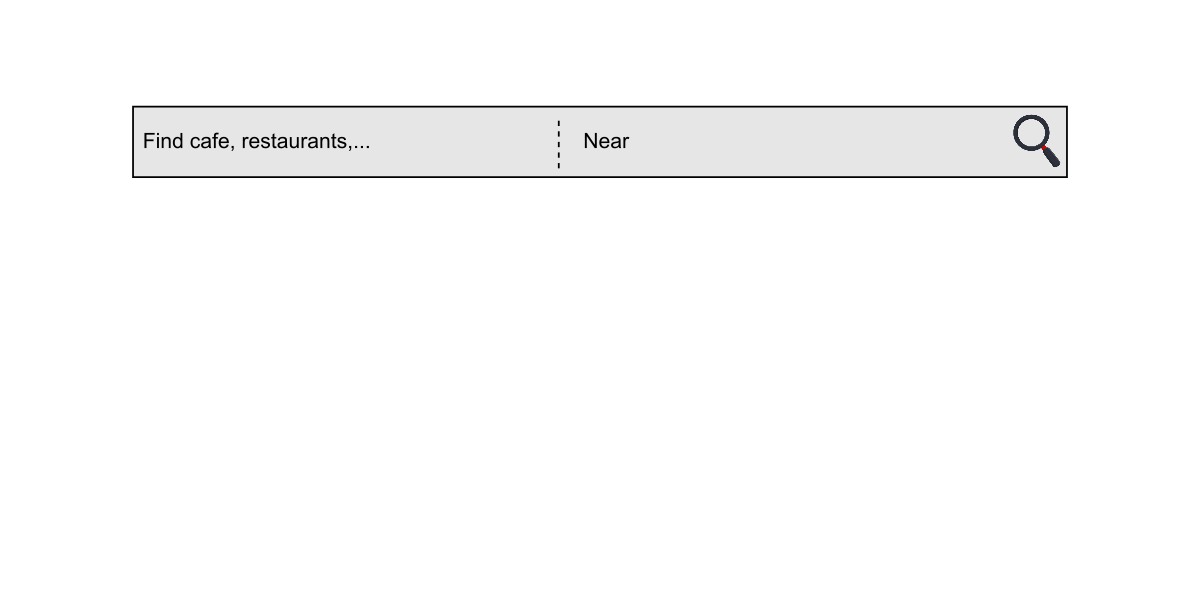
\includegraphics[width=\textwidth]{Images/chapter_29/section_5264443638546432/5627559249444864.png}
 \caption{The user can search for a specific place near them}
 \end{subfigure}
 \hfill
 \begin{subfigure}[b]{0.48\textwidth}
 \centering
 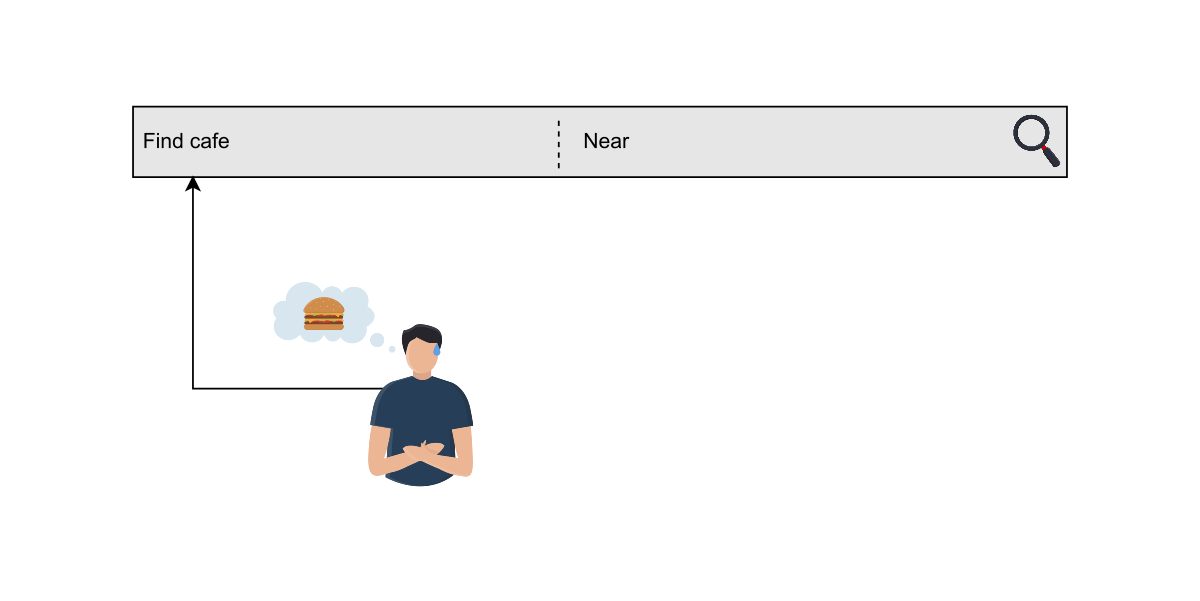
\includegraphics[width=\textwidth]{Images/chapter_29/section_5264443638546432/4661274327908352.png}
 \caption{A user enters “cafe” as their input}
 \end{subfigure}
\end{figure}

\begin{figure}[htbp]
 \centering
 \begin{subfigure}[b]{0.48\textwidth}
 \centering
 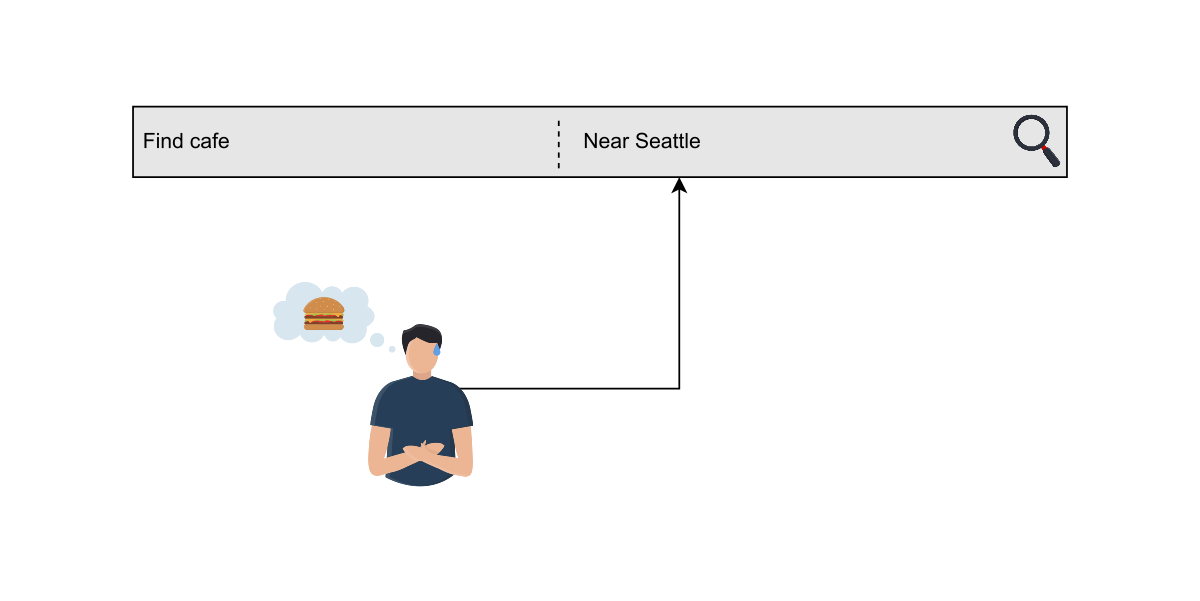
\includegraphics[width=\textwidth]{Images/chapter_29/section_5264443638546432/6641969497636864.png}
 \caption{A user wants to search for cafes around Seattle}
 \end{subfigure}
 \hfill
 \begin{subfigure}[b]{0.48\textwidth}
 \centering
 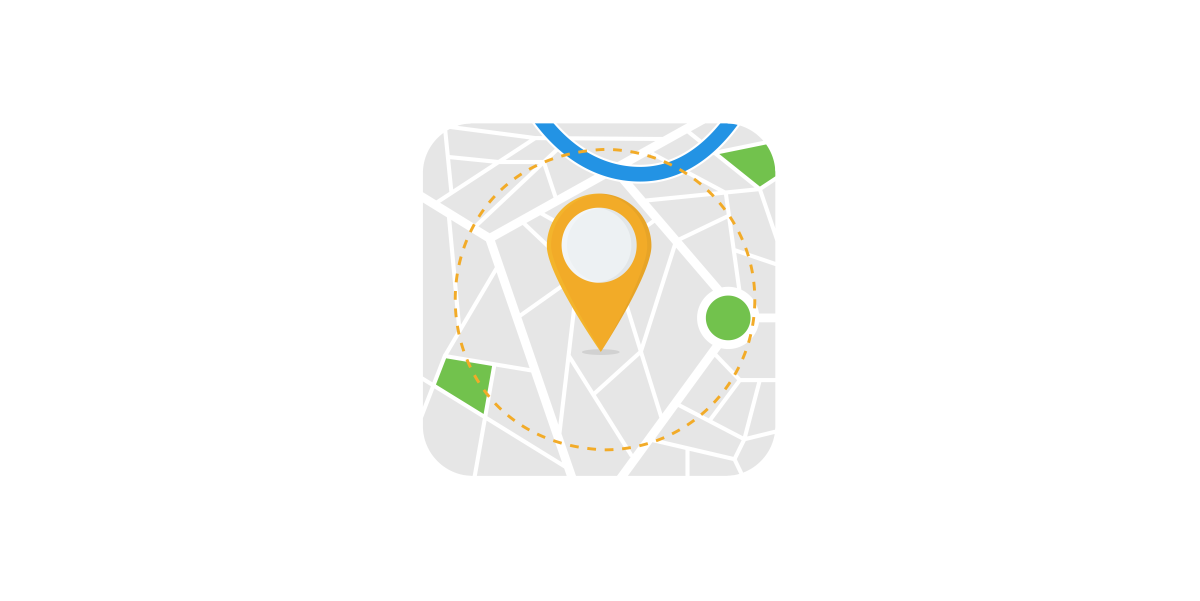
\includegraphics[width=\textwidth]{Images/chapter_29/section_5264443638546432/5316727206576128.png}
 \caption{The proximity server will search for the places in a given radius, keeping user's location as centre point}
 \end{subfigure}
\end{figure}

\begin{figure}[htbp]
 \centering
 \begin{subfigure}[b]{0.48\textwidth}
 \centering
 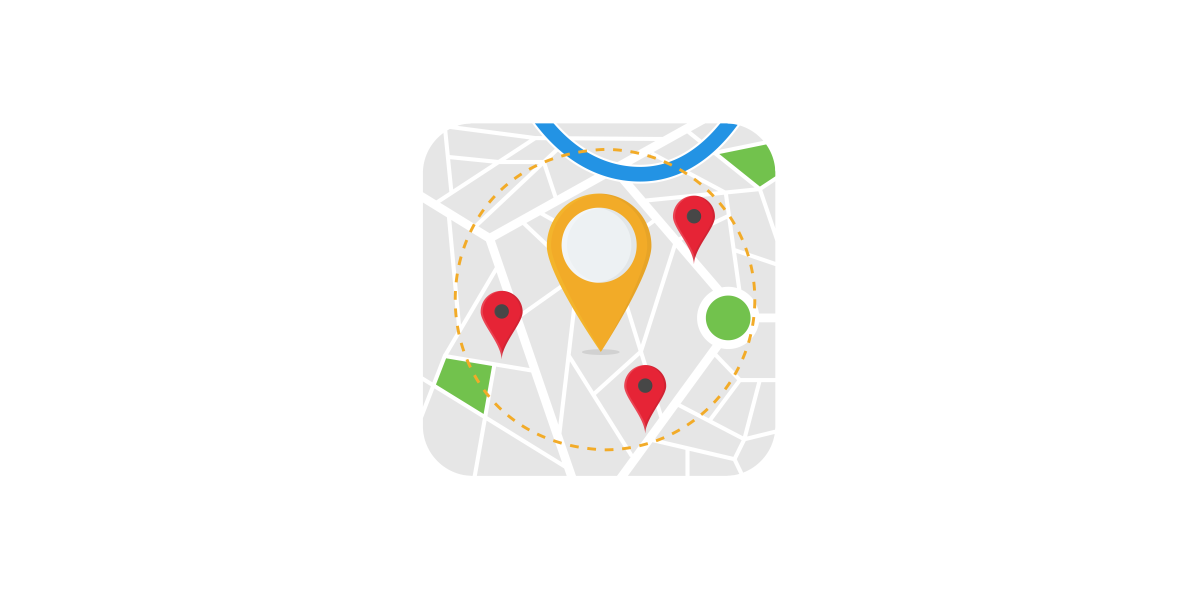
\includegraphics[width=\textwidth]{Images/chapter_29/section_5264443638546432/5608447089573888.png}
 \caption{The proximity server will identify possible places that fit the user’s input}
 \end{subfigure}
 \hfill
 \begin{subfigure}[b]{0.48\textwidth}
 \centering
 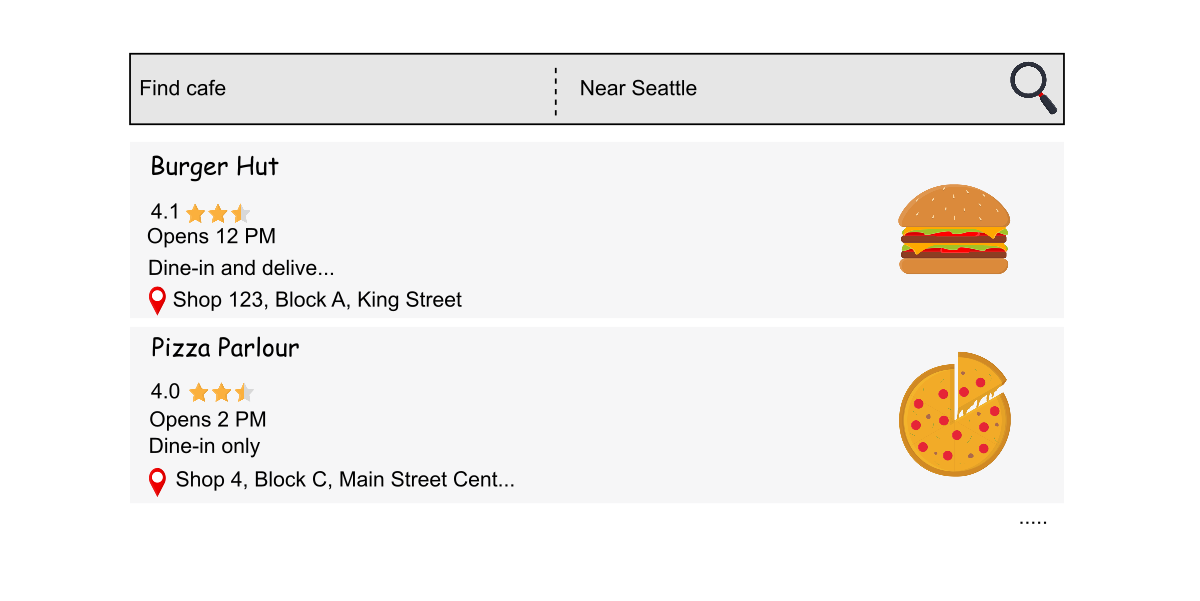
\includegraphics[width=\textwidth]{Images/chapter_29/section_5264443638546432/5881806419394560.png}
 \caption{The proximity server will return the relevant places around Seattle to the user}
 \end{subfigure}
\end{figure}

\subsection{How will we design Yelp?}\label{Je8MGe1cn2it-XhzUcifr}
\\
Here is the breakdown of Yelp's design:

\begin{enumerate}
\item
\protect\phantomsection\label{ar9ZfVuuTuerOlWhSf6Pf}
\href{https://www.educative.io/courses/grokking-the-system-design-interview/requirements-of-yelps-design}{\textbf{Requirements}}: In this lesson, we define the requirements and estimate the required servers, storage, and bandwidth of our system.
\item
\protect\phantomsection\label{VF8xYF-6mTMvOguzhFjVs}
\href{https://www.educative.io/courses/grokking-the-system-design-interview/design-of-yelp}{\textbf{Design}}: In this lesson, we define the API design, the database schema, the components of our system, and the workflow of Yelp.
\item
\protect\phantomsection\label{mM_-kdUQZ_fox_2fT0ONr}
\href{https://www.educative.io/courses/grokking-the-system-design-interview/design-considerations-of-yelp}{\textbf{Design considerations}}: In this lesson, we dive deep into the design of the Yelp system.
\item
\protect\phantomsection\label{IFSJRf4ROmQ-cJ8gC4KXs}
\href{https://www.educative.io/courses/grokking-the-system-design-interview/quiz-on-yelps-design}{\textbf{Quiz}}: In this lesson, we take a quiz to test our knowledge of Yelp design.
\end{enumerate}
\\
Let's start our design by defining its requirements.

% End of section content